% Usar el tipo de documento: Artículo científico.
\documentclass[11pt,a4paper]{article}

% Cargar mensajes en español.
\usepackage[spanish]{babel}

% Usar codificación utf-8 para acentos y otros.
\usepackage[utf8]{inputenc}
\usepackage[T1]{fontenc}
\usepackage{lmodern}

%Dimensiones de los márgenes.
%\usepackage[margin=1.5cm]{geometry}

% Insertar porciones de código
\usepackage{listings}

% Comenzar párrafos con separación no indentación.
\usepackage{parskip}
%enlaces
\usepackage{hyperref}
% Usar gráficos
\usepackage{graphicx}
\usepackage{caption}
\usepackage{subcaption}
%
% Usar contenedores flotantes para figuras.
\usepackage{float}

% Carpeta de las imágenes.
%\graphicspath{{img/}}



%Gummi|065|=)
\title{\textbf{\emph{Deeper.} Bienvenido al futuro}}
\author{rodrigo.arias@udc.es}
\date{}




\begin{document}

\maketitle

\section{Introducción}
\subsection{Expectantes}

Al fin y al cabo un videojuego es quizás la realización más atractiva que uno pudiera 
plantearse al producir gráficos en un ordenador.

Introduce al sujeto en una nueva realidad, provocando que experimente nuevas 
situaciones que han sido cuidadosamente elaboradas. Con el mero propósito de 
causar una sensación sin igual, sin precedentes.

Las cualidades son bien conocidas. Lugares exóticos que no podrían ocurrir en el 
mundo actual. Al menos no en nuestra época. Un sueño donde somos conscientes.  

A todos nos encanta viajar. Experimentar las costumbres de otros lugares.  
Olvidarnos por un segundo de nuestra pequeña burbujita y emprender una aventura.  
Sin conocer el final. Expectantes.

Entonces la modernidad de una época, junto a la intriga más profunda, trastoca 
el significado de la antigua palabra para incluirla en el eje temporal. Que 
ocurriría si pudiesemos hacerlo. Viajar en el tiempo.

Paradojas, dicen los expertos. Pero eso no sacia nuestra curiosidad. No nos 
detiene. Veámoslo con nuestros propios ojos.

\subsection{La máquina}

Es preciso una máquina. Un dispositivo no mucho más grande que una caja donde 
cabe una persona. Un temporizador permite ponerla en funcionamiento de forma programada.

El funcionamiento es bastante sencillo. Aunque sus consecuencias no lo son 
tanto.

Primero activa el temporizador para programar el encendido de la máquina.  
Debes anotar el momento exacto en el que la máquina será activada. Llamaremos a 
este instante el momento A. Asegúrate de que tienes tiempo suficiente para salir 
de ahí, pues no quisieras encontrarte con quien tú sabes.



Aléjate, y realiza las tareas que desees mientras dejas que la máquina se 
encienda sola. Cuando estés listo, prepárate para entrar en la misma. Anota el 
momento exacto en el que entras en la máquina. Este será el momento B.

La máquina te llevará de vuelta al momento A. En ese instante existirán dos 
versiones de tí mismo.

Mantén especial cuidado en no modificar la conducta que has realizado antes de 
entrar en la máquina. Si lo haces, las consecuencias son inciertas. 

\subsection{Consecuencias}

Y entonces, ¿que ocurriría? El juego permite realizar viajes en el tiempo y 
observar los efectos que provoca. Permite aprovechar las ventajas de viajar en 
el tiempo, para poder resolver una serie de escenas.

En cada escena deberás alcanzar un lugar determinado para continuar. Para ello, 
utiliza los objetos que encuentres, y usa tu imaginación e ingenio para resolver 
el rompecabezas.

\subsection{Ambientación}
La idea de las máquinas y su funcionamiento, son de la película Primer, de Shane 
Carruth.

Se han modificado ligeramente. En ella, el sujeto debía permanecer en la 
máquina, un tiempo proporcional al que quería viajar hacia atrás en el tiempo.  
Sin embargo, en el juego, el viaje al pasado ocurre de manera espontánea.


\subsection{Mecanismo de tiempo}
El tiempo que conocemos transcurre de forma lineal. Todo suceso que se produce, 
es debido a unas causas posteriores.

La introducción de una máquina capaz de teletrasportar a una persona al pasado 
lo cambia todo. Para poder referirse a la misma persona en ejes temporales 
diferentes, se incluiye un número que la identifica en un eje temporal concreto.

Cada vez que viajas en el tiempo, el eje temporal se divide en dos partes.

Veamos un ejemplo del mundo cotidiano. Al comienzo, tu número es el 1, y aún no 
has realizado ningún viaje temporal. Entonces decides probar a viajar en el 
tiempo. Para ello has de encender una máquina.

La programas y tras un rato se encenderá. Después de programarla te diriges a 
una cafetería y te tomas un café. Luego, irás a trabajar como todos los días, 
donde pasarás el resto del día, hasta la noche.

Al volver, la máquina ya se encuentra encendida, y puedes usarla. Al meterte 
dentro, la máquina te transporta al pasado, en el momento exacto en el que se 
encendió, cuando te encontrabas desayunando en la cafetería. Tras viajar, el 
número que se te había asignado, ha aumentado. Ahora tu número es el 2.  
Entonces te diriges a la cafetería. Allí, tu versión 1 se encontrará desayunando 
y decides sentarse muy alejado.

Mientras desayunabas, siendo 1, no pensabas en absoluto que tú mismo estuvieras 
ahí en la cafetería, pues fue una decisión que tomaste despues. El efecto de 
aparecer en la cafetería, ocurre antes que las causas, la decisión de ir a la 
cafetería. Y es algo que tendrás que tener en cuenta para poder viajar en el 
tiempo.

En el juego, puedes acercarte tanto como quieras a tu doble, la versión 1, pero 
no puedes tocarlo. Si lo haces, un mecanismo de protección te echará fuera del 
eje temporal, y te devolverá al comienzo del nivel.

Veamos que más puede ocurrir. Siendo 2, te levantas, y vas a donde habías 
aparcado tu coche, y rompes todos los cristales. Es algo que no ocurrió en el 
pasado, y por lo tanto, estás alterando los hechos.

Cuando 1 vaya a subirse para ir al trabajo, el estado del coche, ya no será el 
mismo. Esto no debe ocurrir, ya que estarías cambiando el transcurso del pasado.  
El juego dispone de un mecanismo, que protege a todos los objetos. Si detecta 
que uno no se encuentra en el mismo estado, te devuelve al comienzo.

Estos problemas, se pueden evitar, si sigues las reglas de viajes temporales de 
Shane Carruth, adaptadas a este juego:

\begin{enumerate}
\item Planifica tus viajes primero.
\item No toques la máquina después de salir de ella, tu doble la usará.
\item Cuando compartas el tiempo con tu doble, mantente alejado de él.
\item Preocúpate primero por tí. El presente es el único momento que tiene 
sentido.
\item No seas curioso con lo que te rodea.
\end{enumerate}

\section{Historia}

No existe un futuro establecido. El personaje aparece en un escenario sin saber 
muy bien ni el objetivo, ni lo que debe hacer. Pero poco a poco descubre que las 
máquinas que le proporcionan los viajes en el tiempo para resolver el nivel, son 
las mismas que lo transportan al siguiente.

El juego describe una historia invertida. Un viaje en el tiempo, pero al pasado.  
Cada nivel es un paso más en la historia. Este hecho es el que le pone nombre al 
juego.

El creador de la máquina, ya era muy consciente de lo que ocurriría si encendía 
la máquina por primera vez. Los posibles viajes desde el futuro eran 
impredecibles.  De modo que decidió elaborar una serie de puzzles, de forma que 
sólo él pudiera volver al pasado, al momento en el que construía la máquina.

Todo un ingenioso mecanismo que impedía que un extraño pudiera alcanzar el 
momento cero, el punto en el que la primera máquina se encendía. De forma que 
sólo él se podría impedir a sí mismo la activación de las máquinas iniciales.

Mientras se cubría las espaldas, no se daba cuenta de lo importante que 
resultaría mantenerse con vida. Sólo él conocía los complicados laberintos, que 
permitían el control ilimitado de las máquinas.

Pues tan sólo tres máquinas modulares, permiten realizar infinidad de copias, 
realizando viajes consecutivos al pasado. Para ello, es necesario introducir dos 
máquinas y una persona (el creador) dentro de una misma máquina. Luego salir en 
el pasado, y repetir el procedimiento eligiendo una máquina anfitriona, de las 
dos que se han portado. Entonces las dos máquinas pueden volver al pasado y 
reutilizarse.

La tercera máquina que no se emplea, es la que se observa en el nivel, ya que 
aparece disponible para el jugador. El mundo que se observa en el juego, no es 
más que la misma máquina, colocada por el creador en lugares determinados en un 
tiempo concreto.

El objetivo del juego es llegar al momento cero. El punto en el que se 
encendieron las máquinas por primera vez. Para ello has de resolver el complejo 
laberinto que el creador había ideado. Él por desgracia, ya no puede hacerlo, ni 
ningún otro ser vivo. Los viajes en el tiempo pueden tener consecuencias 
desastrosas, por ello has de impedir la activación de las máquinas, y su 
proliferación.

\subsection{Diagramas}

Para la representación de los viajes en el tiempo, se ha empleado una versión de 
los diagramas de Feynman para la evolución de las partículas con el tiempo. Pero 
adaptados a los viajes temporales. En el eje horizontal se representa el tiempo, 
y en el vertical una posición del espacio.

\begin{figure}[htp]
\centering
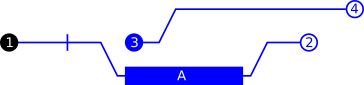
\includegraphics{cronograma1.png}
\caption{Diagrama del primer nivel}
\label{}
\end{figure}

Se recomienda el uso de este tipo de diagramas para la resolución de los
niveles. Sobre todo aquellos que impliquen varios viajes en el tiempo.

En el punto 1, el personaje se encuentra frente a una máquina apagada. La marca 
vertical indica que programa la máquina. Luego se dirige a otro lugar, 
representado como una variación en el eje vertical, y acciona la palanca A. La 
palanca activa una plataforma, que usará para cruzar una zona.

La mantiene accionada un tiempo, y luego vuelve a la máquina, en el punto 2. Se 
introduce en ella y viaja al pasado (hacia la izquierda) hasta el momento en el 
que se encendió la máquina, el punto 3. Un poco después de haberla programado 
(la línea vertical).

Entonces emplea la plataforma activada por la palanca para llegar al punto 4, 
donde se finaliza el nivel.

\section{Diseño interno del juego}

El juego está diseñado por partes conceptuales. Cada objeto se representa en una 
clase. A continuación se mencionan las más importantes del juego. Están 
ordenadas por categorías:

\begin{itemize}
\item Propiedades físicas: Que rigen el comportamiento de los objetos.
\item Objetos: Aquellos que se observan en el nivel.
\item Sistemas de control: Manejan el control del juego y los viajes en el 
tiempo.
\item Lógica del juego: Incluyen los cambios de nivel y diferentes escenas.
\end{itemize}

\subsection{Propiedades físicas}

\subsubsection{SpriteT y Gravity}

Esta clase, permite añadir a un objeto la representación del tiempo, de la 
posición, velocidad y aceleración. Junto con la clase Gravity, que simula el 
efecto de la gravedad, permiten elaborar los movimientos del personaje. Los 
objetos que deseen obtener esta característica, tan sólo han de heredar esta 
clase.

Es importante mencionar que los objetos mantienen una posición absoluta.  
Empleando el eje cartesiano habitual (X positivo hacia la derecha e Y positivo 
hacia arriba). Sin embargo en pygame el eje Y se encuentra invertido, por lo que 
se ajusta antes de colocarse en la escena.

Además, el juego está diseñado para poder ser independiente de los cambios en la 
duración de actualización de fotogramas (framerate). Para ello representa el 
tiempo de los objetos de forma real. Maneja el tiempo de reloj de la CPU, y 
actualiza las posiciones conforme avanza el tiempo real.

Sin embargo, en un videojuego 2D, donde se ha optado por no emplear 
antialiasing, se aprecia una mejor visualización empleando un espacio discreto.  
Ya que los personajes se mueven de forma homogénea. Para ello, la fuente 
temporal es incrementada en una unidad al cambiar de fotograma.

\subsubsection{Collider}
Para gestionar la colisión de un objeto con otro, se emplea la clase Collider.  
Permite añadir la propiedad al objeto que la implemente. OM usará el método 
collide para determinar si el objeto colisiona o no con el personaje.

Se emplea en el suelo y en las plataformas.

\subsection{Objetos}

\subsubsection{Machine}

La máquina es uno de los objetos más complejos. La parte más destacada quizás 
sea su control de las incoherencias. Esto es, una acción que se produce en el 
presente, y que modifica un estado del pasado.

Cuando la máquina detecta esta clase de problemas, efectúa un aviso de 
emergencia que detiene el transcurso del juego y reinicia el nivel.

Por otra parte, las máquinas han sido cuidadosamente elegidas, para que se 
bloqueen en el caso de ser utilizadas. Los bloqueos sirven para prevenir 
incoherencias. Se ha tratado de reducir los bloqueos al mínimo, para que el 
jugador tenga la máxima libertad de elección.

Cuando una máquina se enciende, y a continuación se utiliza, se retrocede al 
pasado, y la máquina queda bloqueada, de forma que sólo el personaje que la 
encendió pueda introducirse en ella. Los demás clones no pueden alterarla.  Ni 
siquiera el jugador activo puede alterar su estado.

Sin embargo, las máquinas que hayan sido encendidas, pero no usadas, no son 
bloqueadas, permitiendo su uso incluso tras haber viajado en el tiempo.

\subsubsection{Boy}

El personaje está representado por la clase Boy. Se emplea esta clase para el 
personaje que está activo, el que recibe los eventos del teclado y reacciona en 
tiempo real. Y también para los duplicados que realizarán acciones del pasado de 
forma programada.

Emplea las propiedades de SpriteT y Gravity. Además es quien guía la cámara, 
cuando es el personaje activo.

Cuando el personaje está desactivado, por pertenecer a una grabación del futuro 
que aún no ha comenzado, este no se muestra en pantalla. La variable disabled 
gestiona este estado.

Una observación con respecto a la actualización del juego. Cuando se recalculan 
las posiciones de todos los objetos, por el hecho de desplazar al jugador, 
primero se recalcula la posición del jugador.

Luego se actualizan los demás objetos, incluyendo el suelo. Despues se vuelve a 
recalcular la posición del jugador, ya que puede que ahora esté chocando con el 
suelo. Finalmente se dibuja en pantalla.

\subsubsection{Palancas}
Las palancas proporcionan una forma de interactuar con el entorno. Actúan como 
pulsadores, de forma que al soltarlas o al alejarse vuelven a la posición 
original.

Esta propiedad fuerza a que para mantener los efectos de la palanca durante un 
intervalo, sea necesario mantenerla durante ese intervalo.

\subsubsection{Plataformas}
El juego se basa en la activación de plataformas, mediante las palancas, que 
permiten al jugador acceder a un lugar anteriormente inaccesible.

Para ello reciben eventos de activación o de desactivación, permitiendo el paso 
del personaje.

\subsection{Sistemas de control}

\subsubsection{Clonaciones}

Todos los objetos del mundo (en el juego), implementan los métodos clone y 
restore. Estos permiten obtener toda la información relevante del objeto, y 
restaurarla en el futuro (en realidad en el pasado) respectivamente.

Son muy importantes para poder volver a un punto determinado del pasado, y 
colocar todo objeto en su lugar y en el mismo estado en el que se encontraba.

\subsubsection{Eventos}

Todos los objetos del juego se pueden comunicar entre ellos empleando un sistema 
de mensajes y eventos. EventDaemon recoge los eventos producidos por los 
objetos, y los envía a su destino. Esto es:

\begin{itemize}
\item Eventos generados por el personaje, como realizar la acción. Que es un 
evento puntual, por lo que se colisiona al personaje y se envía a todos los 
objetos involucrados de forma ordenada. Una vez que el evento es atendido, ya no 
se continúa enviando a ningún otro objeto.

\item Eventos dirigidos, que son enviados al objeto destino, ya predefinido.

\item Eventos de teclado, recogidos por EventControl, que son dirigidos al 
personaje activo.
\end{itemize}

\subsubsection{EventControl}
Esta clase se encarga se recoger los eventos de los dispositivos de entrada, y 
filtrarlos. Además si se presiona la tecla de salir, inmediatamente cierra el 
juego.

Se utiliza una sóla instancia compartida en todos los niveles para poder obtener 
los eventos de teclados. Posteriormente se redirige tanto al jugador activo, 
como a las escenas de pausa.

\subsubsection{LogicConnector}
Esta clase permite añadir un objeto abstracto, que puede tener múltiple entradas 
y salidas. Se emplea para redirigir los eventos. Todos los eventos que son 
recibidos en la entrada, son transmitidos a todos los objetos situados en la 
salida.

De esta forma un objeto como una palanca, puede enviar un evento a dos 
plataformas de forma cómoda.

\subsubsection{ObjectManager}

Todos los objetos son registrados por OM (Object Manager). De forma que para 
realizar una actualización de fotograma, secuencialmente va ejecutando el método 
update de los objetos.

Además gestiona las colisiones del personaje con paredes o suelo, y con otros 
objetos.

Para poder depurar el juego, a mayores se incluye en cada objeto un 
identificador numérico, que es asignado por OM, de forma secuencial.

\subsubsection{Camera}
Dado que el personaje activo recibe el seguimiento de la vista del observador, 
todos los objetos dependen de su posición.

Para ello se ha ideado el mecanismo de cámara, que actualiza un valor de 
desplazamiento conforme a la posición del jugador.

Luego, los objetos piden a la cámara su posición en pantalla, donde se 
dibujarán.

De esta forma, la cámara puede cambiar el objeto al que sigue, y el resto de 
objetos, actualizarán sus posiciones en pantalla de acuerdo con la nueva 
información.

\subsubsection{Grabaciones}

Recording es la clase encargada de ir almacenando las teclas que se presionan 
mientras se juega, y que son enviadas al jugador activo.

Cuando viajas al pasado, la grabación se pone en marcha, y comienza a repetir 
las mismas pulsaciones que se produjeron en el pasado sobre tu personaje, de 
forma que actúa exactamente igual que lo hizo previamente.

Su funcionamiento es idéntico al de una cinta de audio. Primero se coloca en la 
posición inicial y se inicia la grabación. Al terminar, se rebobina la cinta, y 
se inicia de nuevo, esta vez reproduciento el contenido grabado.

Por otra parte en cada viaje, se crea un personaje activo nuevo, y se pone en 
marcha una nueva grabación, que captará los eventos de teclado que se accionen.

\subsubsection{SVT}

La clase SVT (Sistema de Viajes Temporales) es el centro de control del juego.  
Recibe todos los eventos de máquinas y personajes, y realiza los viajes en el 
tiempo oportunos. Esta clase controla el tiempo absoluto, y el tiempo relativo.
El tiempo absoluto es el tiempo en el mundo real, que es creciente y nunca 
retrocede. El tiempo relativo es el que se representa en el juego, y puede 
cambiar al viajar en el tiempo.

Además es la que almacena las grabaciones asignadas a los personajes. Así como 
las copias del mundo en el momento en el que se encienden las máquinas.

Cada máquina dispone del momento exacto en el que se encendió. De forma que al 
accionarla para retroceder al pasado, se calcula la diferencia con el momento 
actual.

Entonces SVT ha de cambiar la hora del juego, y colocarla en el momento en el 
que la máquina se enciende. Esto supone decrementar el tiempo relativo, 
actualizar el tiempo de todos los objetos, recalcular cuales estaban o no en la 
escena, y reproducir las grabaciones oportunas, entre otras acciones.

\subsection{Lógica del juego}

\subsubsection{Level}
Implementa una clase abstracta para el desarrollo de los niveles. Cada nivel 
tiene su SVT, EventDaemon y OM. De forma que se manejan conjuntamente en esta 
clase. Luego cada nivel concreto sólo ha de añadir las diferentes 
configuraciones de objetos a OM.

\subsubsection{GameLogic}

Implementa todo el juego. Se encarga de las escenas, como la de muerte o 
incoherencia, y el avance de los niveles.

Cada nivel informa a GameLogic cuando ha de colocar el siguiente nivel. Los 
niveles se mantienen en una pila, en la que se sobreponen las escenas de 
mensajes como SceneFailure, en la que se indica que el jugador ha perdido y se 
va a reiniciar el nivel.

Cuando ya no quedan más niveles el juego se ha completado.

\section{Limitaciones}
El reto del juego era comprender cómo funcionan los viajes en el tiempo, y que 
implicaciones tendrían.

A lo largo del desarrollo se han ido descubriendo problemas, y se han tratado de 
solucionar, respetando un diseño limpio. Sin embargo, dada la gran complejidad 
que conlleva viajar al pasado, este diseño no es realmente sencillo.

Dado el carácter evolutivo que se ha planteado, quizás el método más apropiado 
para continuar el desarrollo es el de la utilización de prototipos. De forma que 
resulta beneficioso descartar algunas partes, y reescribirlas de una forma más 
sencilla.

Adicionalemente, uno de los problemas de viajar en el tiempo en un entorno 
simulado, es que sólo se puede actualizar un eje temporal a la vez.

Quizás en una interpretación de los viajes en el tiempo más realista, un viaje 
en el tiempo sí permitiría la alteración del pasado. Sin embargo es dificil de 
realizar en un juego. Por ello se incluyen los bloqueos anteriormente 
mencionados. Sin ellos, la coherencia del mundo no está garantizada.

Por otra parte, todo el diseño artístico de ha realizado con grafx2, un programa 
para la edición de píxeles. Sin embargo la gran inexperiencia del autor, deja 
unos resultados muy simples.

\section{Gameplay}

El juego está constituído de varios niveles. Cada uno tiene una complejidad 
mayor que el anterior.

Todos comparten unas características comunes. Dado que el juego es en sí mismo 
un viaje al pasado, se encadenan pequeños viajes para llegar al punto cero. Cada 
nivel es el siguiente eslabón de la cadena de viajes.

Una máquina activa es el punto de partida del nivel, donde aparece el personaje. 
Luego realiza las acciones que le llevan al lugar de la máquina de fin, que le 
permite viajar a siguiente nivel.

\begin{figure}[h]
\centering
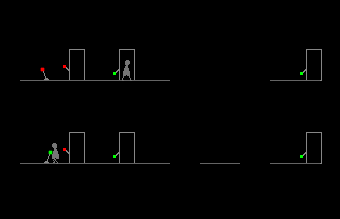
\includegraphics[scale=0.8]{level1.png}
\caption{Dos fotogramas del primer nivel}
\label{fig:level1}
\end{figure}

\begin{figure}[H]
\centering
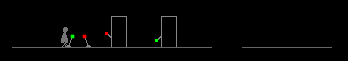
\includegraphics[scale=0.8]{l2.png}
\caption{Nivel 2}
\label{fig:level2}
\end{figure}

\begin{figure}[H]
\centering
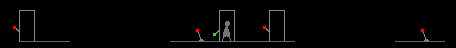
\includegraphics[scale=0.8]{l3.png}
\caption{Nivel 3}
\label{fig:level3}
\end{figure}

\begin{figure}[H]
\centering
\makebox[\textwidth][c]{
	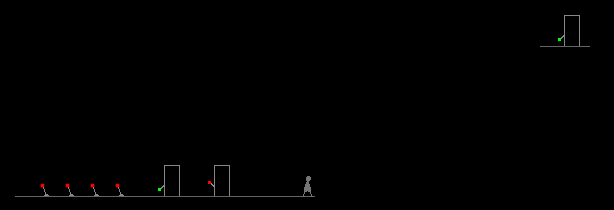
\includegraphics[scale=0.8]{l4b.png}
}
\caption{Nivel 4}
\label{fig:level4}
\end{figure}

\begin{figure}[H]
\centering
\makebox[\textwidth][c]{
	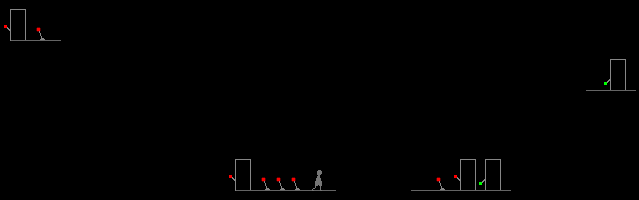
\includegraphics[scale=0.8]{l5b.png}
}
\caption{Nivel 5}
\label{fig:level5}
\end{figure}

Se puede observar que cada máquina proporciona una conexión con el siguiente 
nivel. De hecho, la historia del juego está muy relacionada con cómo se 
resuelven los niveles.

La máquina de comienzo no se puede usar en ningún momento, ya que está 
bloqueada. Dado que será usada en el futuro relativo para llegar al nivel 
actual.

El jugador, no conoce de antemano la historia del juego, y es el hecho de 
emplear las mismas máquinas para viajar en el tiempo dentro del mismo nivel, las 
que han de proporcionarle las pistas suficientes para esbozar la idea de un gran 
viaje al pasado.

\subsection{Contenido de un nivel}
Dado que la gestión común a los niveles se realiza en la clase abstracta Level, 
un nivel tan sólo contiene la disposición de los objetos.

Para ello se van creando los objectos necesarios de forma secuencial. Cada uno 
es colocado en las coordenadas adecuadas. Además han de añadirse a OM, para 
tener un control de los objetos.

Cada nivel debe tener una máquina de inicio, otra de fin, y un personaje.  
Además ha de poder alcanzarse la máquina de fin desde la máquina de inicio.

En la figura~\ref{fig:level1} se muestra como se acciona una palanca que activa 
una plataforma.

\subsection{Escenas}

Al comenzar el juego se muestra una escena de presentación (SceneStart) que 
incluye el título del juego. Al presionar una tecla, se avanza a la siguiente 
escena (SceneControls), que muestra los controles en un resumen. Por último, al 
presionar otra tecla, comienza el juego en el primer nivel.

Existe una escena (SceneFailure) que interrumpe el juego, y que muestra mensajes 
de aviso.  Si el jugador se cae al vacío, se muestra una escena de muerte. Si 
choca con otro jugador (un duplicado), se muestra un mensaje de colisión. Si se 
produce una incoherencia, se muestra el mensaje. Después de esta escena se 
reinicia el nivel.

\section{Cuaderno de bocetos}
Con la entrega de este documento, se adjunta un cuaderno de bitácora, en el que 
se ha ido escribiendo el desarrollo del juego. Así como todos lo problemas que 
se han ido encontrando, sus soluciones, y la explicación necesaria.

Además se incluyen los bocetos de los personajes, los diagramas de los niveles, 
y otras sugerencias que no se han incluído.

Sin embargo, el juego proporciona una buena satisfacción al completar los 
niveles, por lo que se recomienda tratar de resolverlos por uno mismo, y no 
mirar las soluciones.

\section{Ayuda}

\subsection{Controles}
Para mover al personaje, se emplean las teclas de flecha izquierda y derecha, 
que lo desplazan horizontalmente. Para saltar, la flecha hacia arriba. Hacia 
abajo realiza la acción.

Si ha colisionado con un clon, o ha perdido, pulse espacio para volver a 
comenzar.

Finalmente con Q, se cierra el juego. El juego no tiene pausa, de igual modo que 
la vida real no tiene pausas.

\subsection{Ejecución}
Diríjase a la carpeta src, y ejecute: \texttt{python2 main.py}

Requiere las bibliotecas de pygame (probado con la versión 1.9.1-9). Así como la 
versión 2 de python (probado con 2.7.9-1).

Tanto este documento, como el juego, se encuentran en github:

\url{https://github.com/rodarima/pygame}





\end{document}
